\section{Genetic Operators}\label{sec:genetic_operators}
As has been mentioned, genetic operators are applied to members of an existing population to generate a new population. For this assignment the operators used included reproduction, crossover and mutation. As detailed by Koza and Poli \cite{koza2005genetic}, these operators can be briefly summarized as follows:

\begin{itemize}
    \item Reproduction: Copy the selected individual program to the new population as is.
    \item Crossover: Create offspring for the new population by combining randomly chosen parts from two selected programs.
    \item Mutation: Create one new offspring for the new population by randomly mutating a randomly chosen part of a selected individual.
\end{itemize}

Of course, these operators will not be used uniformly to generate new populations. Rather, every operator is associated with a probability which determines the likelihood that it will be used to select the next individual for the new population. In an attempt to determine the most effective probabilities for the operators, 10 tests were run using each of three different combinations of probabilities. The best fitness achieved by each combination is summarized in table \ref{tab:genetic_operator_combinations}.

\begin{table}[H]
\resizebox{\textwidth}{!}{\begin{tabular}{|c|c|c|c|}
\hline
\textbf{Crossover Probability} & \textbf{Reproduction Probability} & \textbf{Mutation Probability} & \textbf{Best Fitness} \\ \hline
0.8                            & 0.1                               & 0.1                           & 9                     \\ \hline
0.9                            & 0.05                              & 0.05                          & 10                    \\ \hline
0.95                           & 0.025                             & 0.025                         & 10                    \\ \hline
\end{tabular}}
\caption{Genetic Operator Combinations}
\label{tab:genetic_operator_combinations}
\end{table}

Following the results of the tests summarized in table \ref{tab:genetic_operator_combinations}, the probability for crossover was selected as 0.8, the probability for mutation was selected as 0.1 and the probability for mutation was also selected as 0.1.

In addition, when applying operators decisions must be made regarding whether to select internal or leaf nodes. The probability for selecting a leaf node was chosen as 0.1 whereas the probability for selecting an internal node was chosen as 0.9.

Finally, a maximum tree depth of 16 was applied as a constraint to the individuals of a new population. In the case of crossover and mutation, the operators would try to produce a valid individual up to 10 times before proceeding to the application of the next operator.

With the selection methods and genetic operators having been identified, figure \ref{fig:breeding_pipeline} depicts the entire breeding pipeline for generating a new population from an existing population.

\begin{figure}[H]
\centering
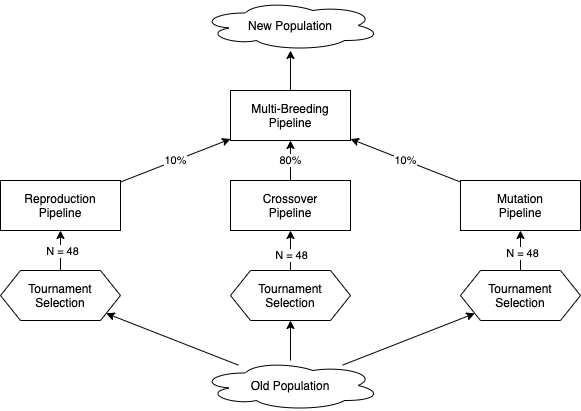
\includegraphics[width=\textwidth]{report/05_genetic_operators/breeding_pipeline.png}
\caption{Breeding Pipeline}
\label{fig:breeding_pipeline}
\end{figure}